% !TEX encoding = UTF-8 Unicode

\documentclass[a4paper]{article}

\usepackage{color}
\usepackage{url}
\usepackage[T2A]{fontenc} % enable Cyrillic fonts
\usepackage[utf8]{inputenc} % make weird characters work
\usepackage{graphicx}
\usepackage{listings}
\usepackage{mathtools}

\usepackage[english,serbian]{babel}

\usepackage[unicode]{hyperref}
\hypersetup{colorlinks,citecolor=green,filecolor=green,linkcolor=blue,urlcolor=blue}

\newtheorem{primer}{Primer}[section]
\newtheorem{definicija}{Definicija}[section]

\begin{document}

\title{Algoritmi za detekciju plagijarizma sa implementacijom algoritma zasnovanog na n-gramima \\ \small{Seminarski rad u okviru kursa\\ Metodologija stručnog i naučnog rada\\ Matematički fakultet}}

\author{Nemanja Subotić, Igor Rodić \\ suboticnemanja93@gmail.com, igorrodic@gmail.com}
\date{2.~maj 2016.}
\maketitle

\abstract{
Sa pojavom modernih tehnologija, pre svega interneta, svet je postao u velikoj meri izložen raznim oblicima zloupotreba. Jednu od tih zloupotreba predstavljaju plagijarizmi. Osnovnu zaštitu predstavljaju računarski algoritmi za detekciju plagijarizma, jer je, s obzirom na količinu dostupnih podataka, za čoveka u velikom broju slučajeva to nemoguće. Tema i cilj rada je prikazivanje osnovnih ideja i pristupa pri impelementaciji ovih algoritama, kao i detaljnijeg opisa i implementacije algoritma za detekciju plagijarizma tekstova na engleskom. Ovaj algoritam zastupa jedan neobičan pristup i u praksi daje dobre rezultate, u nekim slučajevima čak i najbolje.}

\tableofcontents

\newpage

\section{Uvod}
\label{sec:uvod}

Postoje mnoge definicije plagijarizma, ni jedna nije sasvim precizna, pre svega zato što plagijarizam predstavlja nešto drugo za svakoga od nas. Definicija koja stoji u Kembridžovom rečniku (eng.~{\em Cambridge English Dictionary} \cite{cambridge}) glasi:
\begin{definicija}
Plagirati: koristiti tuđe ideje i praviti se da su vaše.
\end{definicija}
\par Osnovu za detekciju plagijarizma predstavljaju računari i efikasni algoritmi koji su u tu svrhu implementirani. U ovom radu čitaocu su predstavljene osnove pisanja algoritama za njihovu detekciju, kao i detaljniji opis algoritma za detekciju plagijarizma teksta, zasnovanog na n-gramima. Prvo su opisane ideje i pristupi, kao i klasifikacija algoritama za detekciju plagijarizma (\ref{sec:ideje i pristupi}). Zatim su u sledećoj sekciji opisani mogući načini sakrivanja plagijarizma, kao i načini da te metode budu otkrivene (\ref{sec:sakrivanje plagijarizma}). Na kraju, implementiran je algoritam teksta zasnovan na n-gramima (\ref{sec:implementacija algoritma za detekciju plagijarizma teksta}).

\section{Sakrivanje plagijarizma}
\label{sec:sakrivanje plagijarizma}

U ovoj sekciji biće reči o tehnikama sakrivanja plagijarizma, sa ciljem težeg otkrivanja, kao i tehnikama za njihovo otkrivanje i prevazilaženje.
\par Kada je u pitanju tekst neke od tehnika za sakrivanje plagijarizma su parafraziranje, korišćenje sinonima, prevođenje na drugi jezik, pa zatim nazad u početni itd. Kada je u pitanju programski kod definisani su nivoi modifikacije koji daju uvid u načine na koje plagijarizam može da bude sakriven \cite{joyluck}:

\begin{itemize}
\item Izmena komentara
\item Izmena belina
\item Preimenovanje identifikatora
\item Izmena rasporeda blokova koda
\item Izmena rasporeda naredbi unutar blokova
\item Izmena redosleda operatora/operanada u izrazima
\item Izmena tipova podataka
\item Dodavanje redundantnih naredbi ili promenljivih
\item Menjanje naredbi kontrole toka ekvivalentnim naredbama kontrole toka (while u do-while itd.)
\item Menjanje poziva funkcije sa telom funkcije
\end{itemize}

Navedene tehnike sakrivanja plagijarizma prevazilaze se pretprocesiranjem. Pretprocesiranje predstavlja modifikovanje fajla pre same primene algoritma za detekciju plagijarizma. U sekcijama \ref{subsec:pretprocesiranje teksta} i \ref{subsec:pretprocesiranje programskog koda} opisane su tehnike pretprocesiranja teksta, i programskog koda.

\subsection{Pretprocesiranje teksta}
\label{subsec:pretprocesiranje teksta}

Tehnike pretprocesiranja teksta su WSD i Thesauri, i parseri. Menjanje reči sinonimima skoro je nemoguće otkriti bez pomoći računara. Na njima se taj problem rešava tokenizacijom, jedan od takvih softvera je i WordNet \cite{fellbaum} (Thesaurus). Ali, pre nego što se uradi zamena svih sinonima jednom rečju, prvo mora biti primenjen WSD (eng.~{\em Word Sense Disambiguation}) metod koji određuje značenje reči u zadatom kontekstu, i tek onda može da bude primenjen tokenizator. Još jedna primena WSD metoda je pri otkrivanju plagijarizma ideje, kada se WSD koristi u kombinaciji sa drvetom konceptualnih klasa, ulazni fajl šalje se na semantičku analizu i dobija se lista klasa, umesto originalnih reči. Lista se dalje procenjuje pomoću uobičajnih algoritama detekcije plagijarizma.

\par Parseri se, sa druge strane, koriste kada je izmenjena struktura teksta (izmenjen redosled reči itd.). Oni dele rečenice na manje sekvence koji oslikavaju strukturu teksta, npr. parser može da prepozna homogene delove rečenice i da ih sortira leksikografski.

\subsection{Pretprocesiranje programskog koda}
\label{subsec:pretprocesiranje programskog koda}

Pretprocesiranje programskog koda deli se na dve tehnike, tokenizaciju i parametrizovano poklapanje. Tokenizacija pretvara programski kod u niz tokena, time ga spuštajući na gradivni nivo (predstavljajući promenljive, pozive funkcija, naredbe itd.) i eliminišući većinu načina skrivanja. Složenost procesa tokenizacije je linearna, stoga ona ne utiče na kompleksnost finalnog algoritma, medjutim, samim procesom mogu da se izgube važne informacije o sličnostima dva programa. U cilju očuvanja te sličnosti tokenizator se koristi zajedno sa parametrizovanim poklapanjem. Parametrizovano poklapanje smatra dva koda identičnim ako jedan može da se dobije iz drugog primenom konačnog broja zamena identifikatora.

\section{Ideje i pristupi}
\label{sec:ideje i pristupi}

Prva stvar o kojoj treba diskutovati jeste klasifikacija sistema za detekciju plagijarizma. Ona je, prirodno, za svakoga drugačija. Osnovna podela, prema Mozgovoju (eng.~{\em Maxim Mozgovoy}) \cite{mozgovoy} deli pomenute sisteme na dve podgrupe, na sisteme koji prave otisak prsta (eng.~{\em fingerprint}) dokumenta i na sisteme koji porede sadržaj \cite{cosma}.

\par Otisak prsta dokumenta predstavlja kratku sekvencu bajtova koja karakterizuje duži dokument. On može da se dobije primenom heš (eng.~{\em hash}) funkcije na dokument, ali obično se koristi niz numeričkih atributa (prosečan broj reči po liniji, prosečan broj ključnih reči itd.), i zatim se pomoću funkcije razdaljine računa stepen različitosti dva dokumenta. Ova tehnika se danas retko koristi jer čak i male promene mogu da rezultuju potpuno drugačijim otiscima.
\par Poređenje sadržaja predstavlja osnovu za veliku većinu sistema za detekciju plagijarizma. Ono je generalno zasnovano na Manberovoj (eng.~{\em Udi Manber}) definiciji sličnosti \cite{manber} i deli se na dve podvrste, na poređenje stringova i na drveta parsiranja.
\begin{definicija}
Manberova definiciji sličnosti: Kažemo da su dva fajla slična ako sadrže značajan broj istih podniski koje nisu prekratke.
\end{definicija}
Algoritmi za poređenje sadržaja funkcionišu po istom principu:
\begin{lstlisting}
FOR EACH collection file F
  FOR EACH collection file G, F =/= G
    Calculate similarity between F and G
\end{lstlisting}
dok se funkcija za određivanje sličnosti menja. Kada pričamo o poređenju stringova pod time podrazumevamo poređenje fajlova, koji se tretiraju kao veliki stringovi. Ovaj način poređenja ne čuva strukturu fajlova, kao ni programskog koda. Algoritmi koji koriste ovaj način detekcije su: FPDS \cite{mozgovoyetal}, koji računa sličnost po formuli:
\begin{lstlisting}
sim(F, G) = MatchedTokens(F, G) / TotalTokens(G)
\end{lstlisting}
YAP \cite{wise} (jedan od prvih algoritama ove vrste, koristi poređenje liniju-po-liniju Levenštajnovim rastojanjem \cite{levenshtein}), RKR-GST koji je implementiran u sistemu YAP3 \cite{wise2} (pravi pokrivač nepreklapajućih stringova koji sadrže maksimalan mogući broj tokena iz oba fajla, algoritam je NP kompletan pa zavisi od uspešnih heuristika, npr. duže podniske su vrednije od kraćih).
\par Drveta parsiranja sa druge strane čuvaju strukturu fajla, kako tekstualnog (poglavlja, pasusi itd.) tako i programskog (klase, funkcije itd.). Prednosti ovog metoda poređenja još nisu u potpunosti iskorišćene, jedan od algoritama koji to pokušava je Sim utility \cite{gitchelltran}. On koristi poređenje stringova, ali ne nad celim fajlovima, već nad njihovim drvetima parsiranja, tj. parser prethodi algoritmu poređenja stringova.

\section{Implementacija algoritma za detekciju plagijarizma teksta}
\label{sec:implementacija algoritma za detekciju plagijarizma teksta}

U ovom delu opisaćemo metod za detekciju pagijarizma tekstova na engleskom jeziku korišćenjem n-grama stop-reči (eng. stopwords). Autor ovog metoda je grčki profesor sa Egejskog univerziteta, Estatios Stamatatos (eng.~{\em Efstathios Stamatatos}) i metod je objavljen 2011. godine \cite{stamatatos}. Pre nego što krenemo sa opisom algoritma, objasnimo prvo osnovne pojmove: n-gram predstavlja niz od n susednih stavki u tekstu, gde stavke mogu  biti karakteri ili reči, dok stop-rečima smatramo najčešće korišćene reči nekog  jezika (u našem slučaju engleskog).  

\par Stop-reči su se pokazale veoma korisnim u istraživanju teksta u slučajevima kad je  bitniji stil pisanja od sadržaja (npr. pripisivanju autorstva i detekcije žanra). Pa tako i profesor Stamatatos predstavlja novi metod detekcije plagijarizma  koji je zasnovan isključivo na strukturnim informacijama. Umesto da eliminiše  stop-reči, kao što je uobičajena praksa, iz teksta eliminiše sve ostale tokene i metod  bazira na preostalom nizu stop-reči. Najčešći način plagiranja je zamena reči i izraza sinonimima. Pošto su stop-reči nezavisne od sadržaja i ne nose nikakve  semantičke informacije, sekvence stop-reči često ostaju nepromenjene prilikom manjih izmena teksta.   

\subsection{Opis algoritma}
\label{subsec:opis algoritma}

Autor je metod podelio na tri dela. U prvom delu se određuje da li je sumnjivi dokument plagijat ili ne. Nakon toga, trebalo bi pronaći sve plagijarizovane delove, odrediti njihove granice i u sumnjivom i u izvornim dokumentima. Na kraju je poželjno  za svaki plagijarizovani deo koji smo pronašli odrediti koeficijent plagijarizma.\cite{stamatatos} 

\par Reprezentacija teksta se zasniva na n-gramima stop-reči (SWNG eng.~{stopword n-gram}). Za dati dokument i listu stop-reči tekst dokumenta se transformiše na sledeći način: prvo se velika slova  prevedu u mala, zatim se vrši tokenizacija i svi tokeni koji se ne nalaze u listi stop-reči se izbacuju, na kraju se grade n-grami. Ovaj skup n-grama stop-reči nazivamo profil dokumenta - \(P(n,d)\). 

\par Profesor Stamatatos kao stop-reči koristi pedeset najčešće korišćenih reči engleskog jezika (\ref{tab:tabela}) prema Britanskom nacionalnom korpusu. 

\begin{table}[h!]
\begin{center}
\caption{50 najčešćih stop-reči u engleskom jeziku.}
\begin{tabular}{|l|l|l|l|l|} \hline
1. the & 11. with & 21. are & 31. or & 41. her \\ \hline
2. of & 12. he & 22. not & 32. an & 42. n't \\ \hline
3. and & 13. be & 23. his & 33. were & 43. there \\ \hline
4. a & 14. on & 24. this & 34. we & 44. can \\ \hline
5. in & 15. i & 25. from & 35. their & 45. all \\ \hline
6. to & 16. that & 26. but & 36. been & 46. as \\ \hline
7. is & 17. by & 27. had & 37. has & 47. if \\ \hline
8. was & 18. at & 28. which & 38. have & 48. who \\ \hline
9. it & 19. you & 29. she & 39. will & 49. what \\ \hline
10. for & 20. 's & 30. they & 40. would & 50. said \\ \hline
\end{tabular}
\label{tab:tabela}
\end{center}
\end{table}

\subsection{Određivanje kandidata}
\label{subsec:odredjivanje kandidata}

Prvi korak je izdvajanje skupa izvornih dokumenata, čiji elementi imaju delove koji su verovatno 
plagijarizovani u sumnjivom dokumentu. Ovo zahteva poređenje sumnjivog dokumenta sa svim izvornim  dokumentima koje imamo kako bi se pronašla bilo kakva lokalna sličnost.

\par Cilj je pronaći zajednički n-gram stop-reči sumnjivog i svakog izvornog dokumenta. Najvažnije je odrediti odgovarajuću vrednost za n, tj. odrediti kolika bi trebala da bude dužina niza uzastopnih stop-reči da bi se otkrila sličnost između  sumnjivog i izvornog dokumenta. Recimo da je to vrednost \( n_{1} \), tada za svaki  zajednički n-gram između para dokumenata gde je \( n < n_{1} \)  poklapanje se smatra neznačajnim, dok za svaki zajednički n-gram između para dokumenata gde je \( n \geq n_{1} \) sugeriše na plagijarizam. Vrednost \( n_{1} \) bi trebala biti relativno visoka, ali trebalo bi imati u vidu da pri znatnim promenama teksta dužina niza uzastopnih reči neće biti velika. 

\par Problem predstavlja slučaj kada se pronađe zajednički n-gram sumnjivog i izvornog dokumenta   koji pripadaju delovima koji su semantički različiti, što uvećava broj lažno pozitivnih plagijarizovanih delova. To je obicno slučaj kada zajednički n-gram sadrži samo veoma česte stop-reči, u engleskom jeziku, to su prvih šest najčešćih stop-reči(the, of, and, a, in, to) i ‘s. Da bi izbegao ovaj slucaj, autor metoda, uvodi ograničenje na sadržaj zajedničkog n-grama. Neka je \( C = \{the, of, and, a, in, to,‘s\} \) skup stop-reči koje se obicno pojavljuju u slučajnim pogocima. Neka je \(D_{x}\) skup sumnjivih dokumenata koje želimo da ispitamo, a \(D_{s}\) skup  izvornih dokumenata i da \(d_{x} \in D_{x}\) i \(d_{s} \in D_{s}\), dok su \(P(n_{1},d_{x})\) i \(P(n_{1},d_{s})\) odgovarajući profili ovih dokumenata koji sadrže n-grame stop-reči dužine \(n_{1}\). Tada je detektovan plagijarizam ukoliko je zadovoljen sledeći kriterijum : 
	\[ \exists g \in P(n_{1}  ,d_{x}) \cup P(n_{1} ,d_{s} ): member(g,C)<n_{1}-1 \land maxseq(g,C)<n_{1}-2 \]
gde je \( member(g,C)\) funkcija koja vraća broj stop-reči n-grama \(g\) koji pripadaju skupu \(C\), a \(maxseq(g,C)\) funkcija koja vraća maksimalnu sekvencu stop-reči u \(g\), koji pripadaju \(C\).

\subsection{Određivanje granica delova}
\label{subsec:odredjivanje granica delova}

Nakon što je pronađen skup izvornih dokumenata koji se poklapaju sa sumnjivim, potrebno je odrediti granice sličnih delova  teksta u svakom od ovih dokumenata. Neka je \( D_{rx} \subseteq D_{s} \) skup dokumenata izdvojenih u prethodnom koraku. Naš cilj je pronalaženje svih \(g\) takvih da je \(g\in P(n, d_{x}) \cup P(n, d_{s})\) pri čemu je \(d_{s} \in D_{rx}\), a nakon toga i građenje sekvenci maksimalne dužine od pronađenih \(g\), tako da svaka dobijena sekvenca predstavlja plagijarizovani deo teksta. Granice delova nam predstavljaju početni i krajnji n-grami u dobijenim sekvencama.  

\par Poklapanje n-grama sumnjivog i izvornog dokumenta može se predstaviti dijagramom rasipanja. Na slici (\ref{fig:slika1}) prikazan je  primer doslovnog plagijarizma, kao i primer plagijarizma nastalog izmenama izvornog dokumenta (\ref{fig:slika2}). Broj praznina i grupa na dijagramu rasipanja zavisi od vrednosti n, tj. reda n-grama korišćenog u kreiranju profila dokumenata. Što je n veće, imaćemo više praznina i grupa.

\begin{figure}[h!]
\begin{center}
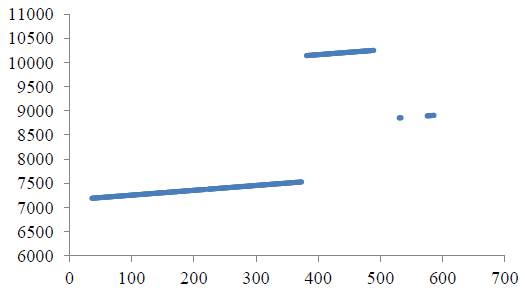
\includegraphics[natwidth=450, natheight=250, scale=0.3]{slika1.PNG}
\end{center}
\caption{Dijagram rasipanja poklopljenih n-grama u slučajevima doslovnog plagijarizma.}
\label{fig:slika1}
\end{figure}

\begin{figure}[h!]
\begin{center}
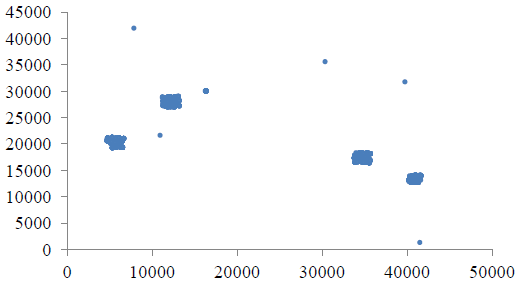
\includegraphics[natwidth=450, natheight=250, scale=0.3]{slika2.PNG}
\end{center}
\caption{Dijagram rasipanja poklopljenih n-grama u slučajevima kada je plagijarizovani pasus pretežno modifikovan.}
\label{fig:slika2}
\end{figure}

\par U prethodnom koraku, da bi utvrdio sličnosti između para dokumenata, autor je koristio duže n-grame (reda \(n_{1}\)), ali za određivanje granica potrebni su mu kraći n-grami (reda \(n_{2} < n_{1}\)) da bi imao detaljnije poređenje. I ovde se dodaje uslov za izbegavanje slučajnih poklapanja n-grama, samo što je uslov malo blaži da bi praznine između zajedničkih n-grama bile manje. Neka su \(P(n_{2}, d_{x})\) i \(P(n_{2}, d_{s})\) profili sumnjivog i izvornog dokumenta koji sadrže \(n_{2}\)-grame stop-reči. Zajednički \(n_{2}\)-gram \(g\) je pronađen ako je zadovoljen sledeći uslov:
 \[g \in P(n_{2} ,d_{x}) \cup P(n_{2} ,d_{s} ): member(g,C)<n_{2}\]
Neka je \(M(d_{x},d_{s})\) skup zajedničkih n-grama između profila P\((n_{2},d_{x})\) i \(P(n_{2},d_{s})\). Na primer, ukoliko je \((17,9) \in M\), to  znaci da sedamnaesti \(n_{2}\)-gram u \(d_{x}\) odgovara devetom \(n_{2}\)-gramu u \(d_{s}\). Članovi skupa \(M\) su poređani na osnovu prvog pojavljivanja u tekstu. Skup \(M\) možemo podeliti na dva dela \(M_{1}\) i \(M_{2}\), tako da odgovaraju, redom, sumnjivom i izvornom dokumentu. Uzastopne vrednosti u \(M_{1}\) su rastuće dok u \(M_{2}\) mogu biti  i opadajuće. Granice plagijarizovanih delova teksta povezane su sa velikim promenama susednih vrednosti u skupovima \(M_{1}\) i \(M_{2}\), što se može videti na slikama (\ref{fig:slika1}) (\ref{fig:slika2}).

\par Pri određivanja granica problem nam može predstavljati slučaj kada imamo više plagijarizovanih delova teksta koja su relativno  blizu, dok su odgovarajući originalni delovi u izvornom dokumentu udaljeni, kao i suprotno. U opisu metoda, predloženo je sledeće rešenje \cite{stamatatos} : Prvo odrediti početni skup granica u sumnjivom dokumentu, tj. podeliti skup M na osnovu razlika susednih vrednosti u M1, pri čemu su dozvoljene manje praznine. Zatim, granice u izvornom dokumentu odrediti tako što se dobijeni  skupovi podele na osnovu razlika susednih vrednosti u \(M_{2}\), gde bi takođe trebalo dozvoliti manje praznine. I na kraju konačni  skup granica u sumnjivom dokumentu odrediti na osnovu dobijenih granica u izvornom dokumentu.    

\subsection{Određivanje koeficijenta plagijarizma}
\label{subsec:odredjivanje koeficijenta plagijarizma}

Svaka detekcija plagijarizma može se predstaviti kao uređena četvorka \( <t_{x}, d_{x}, t_{s}, d_{s}>\), gde \(t_{x}\) predstavlja  plagijarizovan deo teksta u sumnjivom dokumentu \(d_{x}\), koji odgovara delu teksta \(t_{s}\) u izvornom dokumentu \(d_{s}\). Da bi odredio  koeficijent plagijarizma, autor metoda, koristi karakterske n-grame. Prvo se vrši normalizacija delova \(t_{x}\) i \(t_{s}\), tako što se  sva velika slova zamene malim i izbace svi interpunkcijski znaci. Zatim se sličnost između njih računa po sledećoj formuli:
\[ Sim(t_{x}, t_{s}) = \frac{|P_{c}(n_{c}, t_{x}) \cap P_{c}(n_{c}, t_{s})|}{max(|P_{c}(n_{c}, t_{x})|,|P_{c}(n_{c}, t_{s})|)} \]			
gde su \(P_{c}(n_{c},t_{x})\) i \(P_{c}(n_{c},t_{s})\) karakterski \(n_{c}\)-grami profili delova \(t_{x}\) i \(t_{s}\). Izbor vredonsti za \(n_{c}\) zavisi od toga koliko želimo da merenje bude fleksibilno. Što su duži karakterski n-grami to je veća verovatnoća da se izmene neće detektovati kao plagijarizam.

\subsection{Prednosti, rezultati i parametri}
\label{subsec:Prednosti, rezultati i parametri}

Profesor Stamatatos navodi da nije moguće odrediti jedinstvenu vrednost dužine n-grama koja daje najbolje rezultate, ona zavisi od toga šta nam u konkretnom slučaju treba, kao i od raspoloživih resursa (snage računara, memorije itd.). Nakon potpune implementacije algoritma testirano je kako različite dužine n-grama utiču na rezultate detekcije plagijarizma. Testirane su samo različite vrednosti za n jer se pokazalo da menjanje vrednosti m (granice za rupe u plagijatu) ne utiče presudno na rezultate. Takođe, bez obzira na vrednost n, dokumenti koji nisu plagijati su tako i okarakterisani, te nisu uneti u tabelu sa rezultatima (\ref{tab:tabela2}). Iz tabele se vidi da je 8 otprilike prelomna granica za detekciju, i da bi to bio dobar izbor za n.

\begin{table}[h!]
\begin{center}
\caption{Rezultati primene algoritma sa n-gramima.}
\begin{tabular}{|c|c|c|c|c|c|c|} \hline
n & 100\_plag & 80\_plag & 60\_plag & 40\_plag & 20\_plag & modified\_plag \\ \hline
6 & 100\% & 83.9506\% & 62.963\% & 41.9753\% & 22.2222\% & 72.8395\% \\ \hline
7 & 100\% & 83.9506\% & 62.963\% & 41.9753\% & 22.2222\% & 72.8395\% \\ \hline
8 & 100\% & 83.9506\% & 62.963\% & 40.7407\% & 22.2222\% & 70.3704\% \\ \hline
9 & 100\% & 82.716\% & 61.7284\% & 39.5062\% & 20.9877\% & 69.1358\% \\ \hline
10 & 100\% & 81.4815\% & 60.4938\% & 38.2716\% & 20.9877\% & 65.4321\% \\ \hline
\end{tabular}
\label{tab:tabela2}
\end{center}
\end{table}

\section{Zaključak}
\label{sec:zakljucak}

Svakim danom broj javno dostupnih dokumenata, a samim tim i broj plagijarizma, sve je veći. Uporedo, razvijaju se i algoritmi za detekciju plagijarizma kako teksta, tako i programskog koda. Algoritam grčkog profesora Estatiosa Stamatatosa zasnovan na n-gramima stop-reči za detekciju plagijarizma teksta je zanimljiv jer uvodi jedan novi pristup, ali i sadrži u sebi neke prethodne. Trebalo bi pokušati modifikovati algoritam i primeniti ga za detekciju plagijarizma programskog koda, kao i uvesti brojne modifikacije koje se tiču vremenske složenosti, jer je mogućnost da se obradi velika količina dokumenata ključni faktor kada su u pitanju algoritmi detekcije plagijarizma.

\addcontentsline{toc}{section}{Literatura}
\appendix
\bibliography{seminarski} 
\bibliographystyle{plain}

\appendix
\section{Dodatak}

Pored ovog rada, u prilogu se nalaze i izvorni kod algoritma koji je implementiran.

\end{document}
